\documentclass[a4paper, 10pt]{article}
\usepackage[spanish] {babel}
\title{Trabajo Practico 2}
\usepackage{floatflt}
\usepackage{tporga2}
\usepackage{caratula}
\usepackage[pdftex]{graphicx}
\usepackage{color}

\setlength{\leftmargin}{2cm}
\setlength{\rightmargin}{2cm}
\setlength{\oddsidemargin}{-1cm}
\setlength{\evensidemargin}{-1cm}
\setlength{\topmargin}{-1cm}
\setlength{\textwidth}{18cm}
\setlength{\textheight}{25cm}

\usepackage{fancyhdr}
\pagestyle{fancy}
\fancyhf{}
\fancyhead [LO,LE]{\scriptsize Trabajo Pr\'actico N$^{\circ}$2}
\fancyhead [RO,RE]{\scriptsize Gonzales, Mancuso, Mataloni}
\fancyfoot[CE,CO]{\thepage}
\renewcommand{\footrulewidth}{0.4pt}

\usepackage[pdftex, bookmarks=true, colorlinks, citecolor=black, linkcolor=black]{hyperref}
\usepackage{multirow}
\usepackage{listings}

\begin{document}


\materia{Organizaci\'on del Computador II}
\submateria{Segundo Cuatrimestre de 2009}
\titulo{Trabajo Practico N$^{\circ}$2}
\grupo{Grupo RET}
\integrante{Gonzales Courtois Matias}{453/07}{curtu\_infinito73@hotmail.com}
\integrante{Mancuso Emiliano}{597/07}{emiliano.mancuso@gmail.com}
\integrante{Mataloni Alejandro}{706/07}{amataloni@gmail.com}
\maketitle
\newpage

\addcontentsline{toc}{section}{\'Indice}
\tableofcontents

\newpage

\section{Enunciado}

Optimizar las funciones de procesamiento de im\'agenes desarrolladas en el primer trabajo pr\'actico. Para eso se debe utilizar el modelo de programaci\'on SIMD (Single Instruction Multiple Data) y el set de instrucciones SSE de la arquitectura IA-32 de Intel. Adem\'as de los operadores de derivaci\'on ya vistos (Roberts, Prewitt y Sobel) para esta nueva entrega se pide implementar tambi\'en el filtro de Frei-Chen (ver Introducci\'on Te\'orica del TP1) que requiere un procesamiento en punto flotante.

Al igual que en la entrega anterior, se debe escribir la parte de interacci\'on con el usuario y manejo de archivos en lenguaje C, utilizando la librer\'ia ́OpenCV. Las funciones de procesamiento de im\'agenes deben estar escritas en lenguaje ensamblador optimizado para instrucciones SIMD. El programa debe recibir en la l\'inea de comandos el nombre del archivo de entrada y la operaci\'on:

\begin{itemize}
\item r1 = realzar los bordes con el operador de Roberts.
\item r2 = realzar los bordes con el operador de Prewitt. 
\item r3 = realzar los bordes con el operador de Sobel, derivaci\'on s\'olo en x.
\item r4 = realzar los bordes con el operador de Sobel, derivaci\'on s\'olo en y.
\item r5 = realzar los bordes con el operador de Sobel, derivaci\'on en x y en y.
\item r6 = realzar los bordes con el operador de Frei-Chen.
\end{itemize}

\newpage

\section{Introducci\'on}

En el trabajo pr\'actico anterior hab\'iamos resuelto los algoritmos de forma tal, que no utilizamos las matrices de los operadores debido a que conoc\'iamos los valores.
Partimos desde este punto para optimizar el procesamiento de im\'agenes con instrucciones SIMD. \\

Pudimos desarrollar los algoritmos facilmente, a excepci\'on de Frei-Chen, que no nos alcanzaban los registros. \\

Quer\'iamos optimizar los accesos a memoria, por lo tanto levantabamos las 3 lineas en 3 registros distintos, y las manteniamos durante todo el ciclo.

\begin{center}
	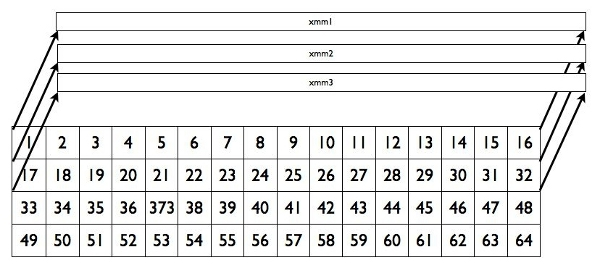
\includegraphics[scale=0.70]{Graficos/graph1.jpg}
\end{center}

Para poder operar entre los pixeles, los desempaquetabamos hasta llegar a enteros de 32 bits, y asi poder multiplicar por $\sqrt{2}$. 
Luego, volviamos a empaquetar a 8 bits para guardar el resultado.
Esto nos consumia todos los registros SSE, y solo hab\'iamos realizado el operador en X. Otra desventaja que tra\'ia es que pod\'iamos procesar de a 6 pixeles, y era dificil de seguir e implementar. \\

La $\sqrt{2}$ siempre la manten\'iamos en un registro \textbf{xmm0} y asi, calcularla solo una vez.
Al no alcanzarnos los registros de SSE, optamos por utilizar variables auxiliares donde contenerla, total el acceso a memoria ocurrir\'ia una sola vez, gracias a la memoria cache. \\

Sin embargo, la implementaci\'on del algoritmo se nos segu\'ia complicando, sobretodo al intentar operar X e Y al mismo tiempo sin pasar por memoria, que es lo \'optimo y a lo que intentabamos llegar. \\

Con este problema fuimos a consultar, y nos aconsejaron que tomemos el problema con otro punto de vista.
En lugar de pensar el problema como sumas horizontales, y mantener los resultados con \textit{shift} y mascaras, deber\'iamos pensar el problema como si se tratase de sumas verticales. \\

As\'i es como lo repensamos e hicimos la nueva implementaci\'on, mucho m\'as clara, m'as eficiente, y con registros SSE suficientes !

\newpage

\section{Implementaci\'on de los algoritmos}

En lugar de levantar las 3 lineas y trabajar con ellas, vamos trabajando de a una linea.

\begin{center}
	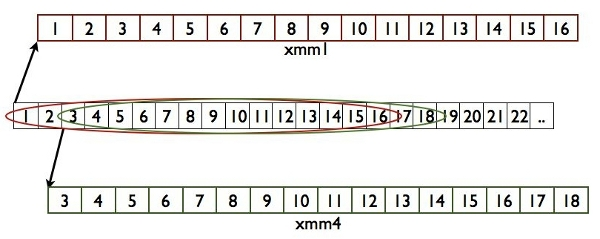
\includegraphics[scale=0.70]{Graficos/graph2.jpg}
\end{center}

Una vez que cargamos la linea en xmm1 y la misma linea pero desplazado 2 pixeles a la derecha en xmm4, hacemos la resta de forma vertical y la mantenemos en xmm1

\begin{center}
	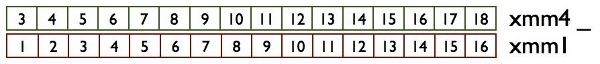
\includegraphics[scale=0.7]{Graficos/graph3.jpg}
\end{center}

Procedemos de la misma manera para la segunda linea, quedando en xmm2 y para la tercer linea, en xmm3.

Ahora que tenemos procesadas cada una de las lineas, las tenemos que sumar entre si, pero sin olvidarnos de que la linea 2 (xmm2) debe ser multiplicado por $\sqrt(2)$.
Para ello, desempaquetamos de a 4 n\'umeros hasta tener enteros de 32 bits, los convertimos en n\'umeros de punto flotante, los multiplicamos por $\sqrt{2}$ y luego los convertimos en enteros, y volvemos a empaquetar hasta obtenerlos en byte. \\


\lstset{language=[x86masm]Assembler}
\begin{lstlisting}
	movdqu xmm4, xmm2
	punpcklbw xmm4, xmm5  ; extendemos a 16 bits los 8 numeros de la parte baja.
	punpcklwd xmm4,xmm5   ; extendemos a 32 bits los 4 numeros de la parte baja.

	cvtdq2ps xmm4,xmm4    ; convertimos a float		
	mulps xmm4,xmm0       ; multiplicamos por raiz(2)
	cvtps2dq xmm4, xmm4   ; lo volvemos a convertir en enteros de 32

	packssdw xmm4,xmm4    ; xmm4 = primeros 4 resultados
	packuswb xmm4,xmm4    ; los devolvemos a byte
\end{lstlisting}

\newpage

Ahora xmm2 contiene los n\'umeros multiplicados por $\sqrt{2}$ listos para ser sumados con los otros.

Por \'ultimo, sumamos con saturaci\'on los tres registros de forma vertical para obtener los resultados y lo asignamos a \textbf{xmm7}. \\ 

Esto es v\'alido dado que:
\begin{center}
	\begin{tabular}{llllllll}
		A & B & C & & & -1 & 0 & 1 \\
		D & E & F & & & -$\sqrt{2}$ & 0 & $\sqrt{2}$ \\
		G & H & I & & & -1 & 0 & 1 \\
	\end{tabular}
\end{center}

\begin{center}
	\entonces - A - D$\sqrt{2}$ - G + C + F$\sqrt{2}$ + I \\
	$\Leftrightarrow$ - A + C - D$\sqrt{2}$ + F$\sqrt{2}$ - G + I \\
	$\Leftrightarrow$ C - A + (F - D)$\sqrt{2}$ + I - G \\ 
\end{center} 


Acerca de los bordes de la im\'agen, hay dos soluciones 
\begin{itemize}
	\item{Agregar un pixel dem\'as en los bordes, ya sea clonandolos o en negro, para hacer posible el calculo de la im\'agen por completo.}
	\item{Ignorar los bordes y dejarlos en negro}
\end{itemize}


Nosotros optamos por ignorar los bordes y dejarlos en negro.

Hasta ac\'a, en \textbf{xmm7} tenemos el resultado de haber procesado la im\'agen con el operador Frei-Chen pero solo en X. \\

Para calcular Frei-Chen en Y, el algoritmo es muy similar, en lugar de tomar la primer fila y su corrimiento de dos pixeles, tomamos la primer fila y la tercera, pues en Y la segunda fila la ignoramos por ser 0. \\ 

Despues se procede de la misma manera.

\section{Imagenes procesadas}

Las im\'agenes procesadas se encuentran en el directorio \texttt{resultados} debido a que el procesamiento de las im\'agenes no se puede apreciar en una impresi\'on.
Hay que ejecutar el programa, para elegir el operador a utilizar y luego alguna de las im\'agenes del directorio \texttt{src/images/}.


\newpage


\section{RET-SIMD vs. OpenCV vs. RET }
En esta secci\'on podemos ver la diferencia entre procesar las im\'agenes con registros de proposito general, y con registros MMX.
Entonces, utilizamos los algoritmos desarrollados en el Trabajo Pr\'actico 1 y los comparamos con los reci\'en explicados.

Adem\'as, aprovechamos y mostramos al mismo tiempo la comparaci\'on con la implementaci\'on de la librer\'ia \texttt{OpenCV}.

De esta forma, podemos ver las 3 implementaciones distintas, agrupadas por operador (X, Y o XY).
La librer\'ia OpenCV implementa su propio algoritmo para el operador de Sobel con registros de pr\'oposito general.
En cambio nosotros, a diferencia de OpenCV, implementamos el algoritmo con instrucciones SIMD.
Para comparar los algoritmos utilizamos im\'agenes de distintos tama\~nos, y medimos los ciclos del CPU para comparar la eficiencia de las distintas implementaciones.

\begin{center}
	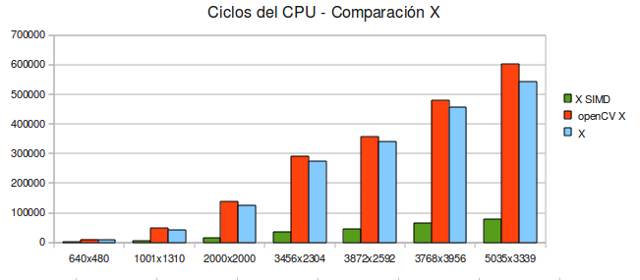
\includegraphics[scale=0.60]{Graficos/comp_X.png}
\end{center}

\begin{center}
	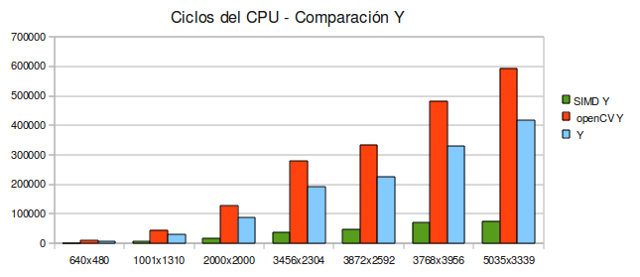
\includegraphics[scale=0.60]{Graficos/comp_Y.png}
\end{center}

\begin{center}
	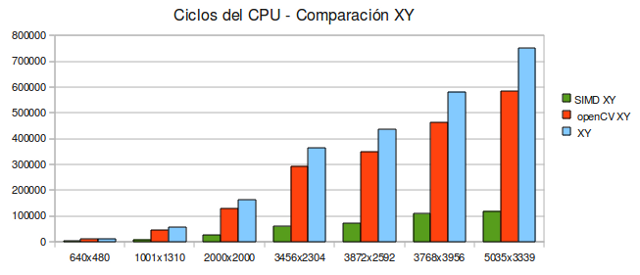
\includegraphics[scale=0.60]{Graficos/comp_XY.png}
\end{center}

Para realizar estos gr\'aficos, seleccionamos distintas im\'agenes con distinta resoluci\'on, y corrimos cada algoritmo un total de 20 veces para luego calcular un promedio.
Para ajustar la escala del gr\'afico, la cantidad de ciclos esta representada en miles, pues sino se hac\'ia despreciable respecto a las im\'agenes m\'as peque\~nas. \\ 

\section{Conclusi\'on}
Gracias a estos gr\'aficos podemos contrastar la velocidad que nos brindan las instrucciones \texttt{SIMD}.
Tambi\'en llegamos a la conclusi\'on de que la librer\'ia \texttt{OpenCV} no utiliza instrucciones \texttt{SIMD}, y esto se debe a que la librer\'ia se utiliza en muchos lugares y no todos los procesadores implementan esta tecnolog\'ia.
Si supieramos que estos algoritmos correr\'ian sobre procesadores IA-32 compatibles con instrucciones SIMD, definitivamente ser\'ia la mejor opci\'on.
Pero, dado que no son los \'unicos procesadores, la librer\'ia prioriza la portabilidad de los algoritmos frente a la optimalidad.
Por eso, tenemos una diferencia abismal entre las distintas implementaciones.

\newpage

\section{Manual de usuario}
\begin{enumerate}
	\item Ejecutar el comando \texttt{make} o \texttt{make install} desde el directorio \texttt{tp2}.
	\item Acceder al directorio \texttt{exe} y ejecutarlo
	\begin{enumerate}
		\item Directo \texttt{./tp r1 images/lena.bmp }
		\item Interactivo \texttt{./tp }
	\end{enumerate}	
	\item Las im\'agenes procesadas se encuentran en el directorio \texttt{resultados}.
	\item En el directorio \texttt{src/images/} se encuentran algunas im\'agenes de ejemplo para procesar.
	\item Para agregar im\'agenes a procesar, estas deben ser agregadas al directorio \texttt{src/images/}.

\end{enumerate}

\section*{Archivos}
\begin{lstlisting}[language=SHELXL]
tp2/
|-- Makefile
|-- enunciado
|   `-- Enunciado.pdf
|-- exe
|-- informe
|   `-- Informe.pdf
|-- resultados
`-- src
    |-- Makefile
    |-- asmFrei_Chen.asm
    |-- asmPrewitt.asm
    |-- asmRoberts.asm
    |-- asmSobelXY.asm
    |-- images
    |   |-- 10mb.jpg
    |   |-- 1mb.jpg
    |   |-- 2mb.jpg
    |   |-- 5mb.jpg
    |   |-- emma.jpeg
    |   |-- foto3.jpg
    |   |-- lena.bmp
    |   `-- pink.jpg
    `-- main.c

\end{lstlisting}

\end{document}
